\documentclass[main]{subfiles}

\begin{document}

\begin{definition}
An \textbf{abstract simplicial complex}\index{abstract simplicial complex} is $K\subseteq \mathscr P(S)\setminus\varnothing$ such that $X\in K\Rightarrow\mathscr{P}(X)\setminus\varnothing\subseteq K$. Finite elements of $K$ are called \textbf{faces}. The \textbf{dimension} of a face $X$ is $\dim X=|X|-1$. The $d$ skeleton $K^d$ is the union of faces of dimension no more than $d$. $\dim K=\displaystyle\sup_{X\in K}\dim X$. $K^0$ are \textbf{vertices}. Maximal elements are \textbf{facets}. $K$ is \textbf{pure} if all facets have dimension $\dim K$. A \textbf{simplex} is a subcomplex which contains all its nonempty subsets, for $X\in K$, $\overline X$ is the corresponding simplicial complex
\end{definition}

\begin{definition}
The \textbf{closure} $\overline L$ of $L\subseteq K$ is smallest subcomplex of $K$ containing $L$. The \textbf{star} of $Y\in K$ is $\st L=\{X|X\cap Y\neq0\}$, the star of $L\subseteq K$ is $\st L=\displaystyle\bigcup_{Y\in L}\st Y$. The \textbf{link} of a face $Y\in K$ is or $\lk Y=\{X|X\cap Y=\varnothing, X\cup Y\in X\}$. Equivalently, $\lk Y=\overline{\st Y}-\st\overline Y$
\begin{figure}[h!]
\centering
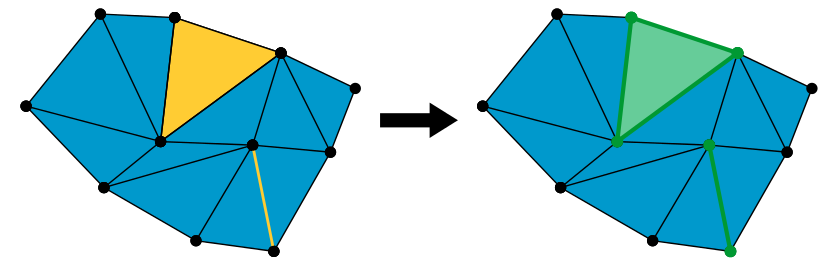
\includegraphics[scale=0.2]{Pictures/Closure_of_a_complex}
\caption{Two \textcolor{yellow}{simplices} and their \textcolor{green}{closure}}\label{Closure of a complex}
\end{figure}
\begin{figure}[h!]
\centering
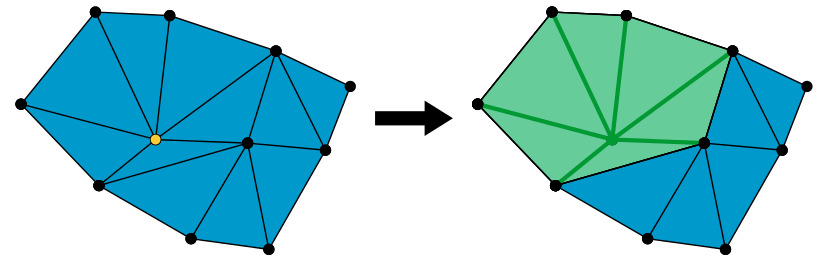
\includegraphics[scale=0.2]{Pictures/Star_of_a_complex}
\caption{A \textcolor{yellow}{vertex} and its \textcolor{green}{star}}\label{Star of a complex}
\end{figure}
\begin{figure}[h!]
\centering
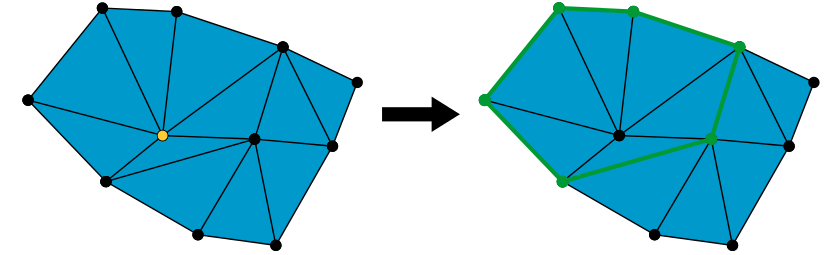
\includegraphics[scale=0.2]{Pictures/Link_of_a_complex}
\caption{A \textcolor{yellow}{vertex} and its \textcolor{green}{link}}\label{Link of a complex}
\end{figure}
\end{definition}

\begin{note}
$\lk\varnothing=K$
\end{note}

\begin{definition}
If $K,L$ has disjoint sets of vertices, then $K*L=\{X\sqcup Y|X\in K,Y\in L\}$
\end{definition}

\begin{definition}
$L\subseteq K$, the \textbf{deletion} $K\setminus L$ consists of those sets which don't contain sets in $L$ as subsets. The stellar subdivision of $X\in K$ is by introducing a new vertex $x$, and form $K\setminus X\cup(\overline x*\partial\overline X*\lk X)$
\end{definition}

\begin{definition}
A simplicial map $f:K\to L$ is such that $f(K^d)\subseteq L^d$
\end{definition}

The Eilenberg-Zilber map $C_*(X)\otimes C^*(Y)\to C^*(X\times Y)$ is a quasi-isomorphism

Take $X,Y=I$
\begin{center}
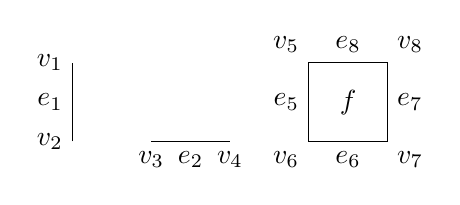
\begin{tikzpicture}
\draw (0,0)node[left]{$v_2$}--(0,1)node[left]{$v_1$};
\node[left]at(0,0.5){$e_1$};
\draw (1,0)node[below]{$v_3$}--(2,0)node[below]{$v_4$};
\node[below]at(1.5,0){$e_2$};
\draw (3,0)node[below left]{$v_6$}--(4,0)node[below right]{$v_7$}--(4,1)node[above right]{$v_8$}--(3,1)node[above left]{$v_5$}--cycle;
\node[below] at(3.5,0){$e_6$};
\node[right] at(4,0.5){$e_7$};
\node[above]at(3.5,1){$e_8$};
\node[left]at(3,0.5){$e_5$};
\node at(3.5,0.5){$f$};
\end{tikzpicture}
\end{center}
The map sends $v_1\otimes v_3\mapsto v_5, v_1\otimes v_4\mapsto v_8, v_2\otimes v_3\mapsto v_6, v_2\otimes v_4\mapsto v_7, e_1\otimes v_3\mapsto e_5, e_1\otimes v_4\mapsto e_7, v_1\otimes e_2\mapsto e_8, v_2\otimes e_2\mapsto e_6, e_1\otimes e_2\mapsto f$. The we get the quasi-isomorphism
\begin{center}\tiny
\begin{tikzcd}
0 \arrow[r] & {\mathbb Z[\{e_1\otimes e_2\}]} \arrow[r] \arrow[d] & {\mathbb Z[\{e_1\otimes v_3,e_1\otimes v_4,v_1\otimes e_2,v_2\otimes e_2\}]} \arrow[r] \arrow[d] & {\mathbb Z[\{v_1\otimes v_3,v_1\otimes v_4,v_2\otimes v_3,v_2\otimes v_4\}]} \arrow[r] \arrow[d] & 0 \\
0 \arrow[r] & {\mathbb Z[\{f\}]} \arrow[r]                        & {\mathbb Z[\{e_5,e_7,e_8,e_6\}]} \arrow[r]                                                       & {\mathbb Z[\{v_5,v_8,v_6,v_7\}]} \arrow[r]                                                       & 0
\end{tikzcd}\normalsize
\end{center}

\begin{definition}\label{Standard simplex}
With the standard basis $\{e_i\}$ for $\mathbb R^\infty$ as vertices, the \textbf{standard} $n$\textbf{-simplice} is
\[\Delta^n=\left\{(t_0,\cdots,t_n)\in\mathbb R^{n+1}\subseteq\mathbb R^\infty\middle|\sum t_i=1,0\leq t_i\leq1\right\}\]
The $i$\textbf{-th face} of $\Delta^n$ is the face oppose to the $i$-th vertex, i.e. $\left\{t_i=0\right\}\cap\Delta^n$ \par
The \textbf{boundary} of $\Delta^n$ to be $\partial\Delta^n$ is the union of faces. $\partial \Delta^0=\varnothing$
\begin{center}
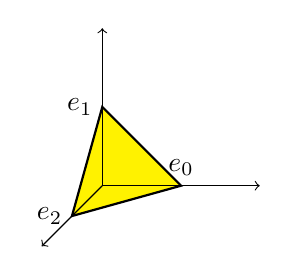
\begin{tikzpicture}
\filldraw[,thick, color=black, fill=yellow] (1,0,0)--(0,1,0)--(0,0,1)--cycle;
\draw[->](0,0,0)--(2,0,0);
\draw[->](0,0,0)--(0,2,0);
\draw[->](0,0,0)--(0,0,2);
\node at (1,0,0)[above]{$e_0$};
\node at (0,1,0)[left]{$e_1$};
\node at (0,0,1)[left]{$e_2$};
\end{tikzpicture}
\end{center}
$\Delta^{n-1}\xrightarrow{d_{n,i}}\Delta^{n}$, $e_j\mapsto\begin{cases}
e_j &j<i \\
e_{j+1} &j\geq i
\end{cases}$ is $i$-th \textbf{face map} attaching $\Delta^{n-1}$ to the $i$-th face of $\Delta^n$ \par
$\Delta^{n+1}\xrightarrow{s_{n,i}}\Delta^n$, $e_j\mapsto\begin{cases}
e_j &j\leq i \\
e_{j-1} &j>i
\end{cases}$ is the $i$-th \textbf{degeneracy map} which is a projection
\end{definition}

\begin{definition}
$X$ has a \textbf{cell decomposition}\index{Cell decomposition} if $X$ can be written as the disjoint union of open $n$ cells, i.e. $\displaystyle X=\bigcup_{n,\alpha}e^n_\alpha$, where cells $e^n_\alpha$ with subspace topology are homeomorphic to open $n$ disks or open $n$ simplices and disjoint, $\displaystyle X^n=\bigsqcup_{k\leq n,\alpha}e^k_\alpha$ is called the $\mathbf{n}$\textbf{-skeleton}\index{Skeleton}, define $X^{-1}=\emptyset$ \par
Suppose $X,Y$ have cell decomposition $\displaystyle X=\bigcup_{n,\alpha}e^n_\alpha$, $\displaystyle Y=\bigcup_{m,\beta}e^m_\beta$, then $X\times Y$ also has a cell decomposition $\displaystyle X\times Y=\bigcup_{k}\bigcup_{\substack{n+m=k \\ \alpha,\beta}}e^n_\alpha\times e^m_\beta$, note that $e^n_\alpha\times e^m_\beta\cong e^{n+m}$ \par
Every topological space has a cell decomposition into points
\end{definition}

\begin{definition}
A \textbf{cellular map}\index{Cellular map} is a map $f:X\to Y$ between topological spaces with cell decompositions such that $f(X^n)\subseteq Y^n$
\end{definition}

\begin{definition}
$X$ is called a \textbf{cell complex}\index{Cell complex} if $X$ is a Hausdorff space with cell decomposition $\displaystyle X=\bigcup_{n,\alpha}e^n_\alpha$ and a cell complex structure: a family of characteristic maps $\Phi^n_\alpha:\Delta^n\to X$ such that $\Phi^n_\alpha$ restricted on $\Delta^n\setminus\partial\Delta^n$ is a homeomorphism onto $e^n_\alpha$ and $\Phi^n_\alpha\left(\partial\Delta^n\right)\subseteq X^{n-1}$ \par
Note that in the definition, we could also replace $\Delta^n$ with $D^n$
\end{definition}

\begin{remark}
Since $\Delta^n$ is compact Hausdorff and $X$ is Hausdorff, $\overline{e^n_\alpha}\subseteq \Phi^n_\alpha\left(\Delta^n\right)$, $\partial e^n_\alpha\subseteq \Phi^n_\alpha\left(\partial\Delta^n\right)$ for $n>0$, on the other hand, if $\partial e^n_\alpha\subsetneqq \Phi^n_\alpha\left(\partial\Delta^n\right)$, then there exists $x\in\partial\Delta^n$ such that $y=\Phi^n_\alpha(x)\notin\overline{e^n_\alpha}$, this means there is an open neighborhood $U$ of $y$ disjoint from $\overline{e^n_\alpha}$, but then the preimage of $U$ under $\Phi^n_\alpha$ would be a nonempty open subset of $\Delta^n$ which intersects $\Delta^n\setminus\partial\Delta^n$ which is impossible, hence  $\Phi^n_\alpha\left(\Delta^n\right)=\overline{e^n_\alpha}$, $\Phi^n_\alpha\left(\partial\Delta^n\right)=\partial e^n_\alpha$ for $n>0$ \par
A Hausdorff space $X$ with a cell decomposition doesn't immediately give a cell complex structure, for example, consider an open disk union with an open segment right in the middle
\begin{center}
\begin{tikzpicture}
\draw (0,0) ellipse (2 and 1);
\filldraw [white] (0,1) circle (0.05);
\draw (0,0)--(0,2);
\end{tikzpicture}
\end{center}
Cell complex $X$ can be seen as
$\Delta^n$ is compact Hausdorff and $X$ is Hausdorff and Lemma \ref{X compact + Y Hausdorff => f:X->Y quotient map}
\end{remark}

\begin{definition}
A cell complex $X$ is called \textbf{regular} if all characteristic maps are embeddings
\end{definition}

\begin{definition}
Let $X$ be a cell complex, it is \textbf{closure finite} if $\overline{e^n_\alpha}$ is contained in the union of finitely many cells, and we say $X$ has the \textbf{weak topology}, meaning $F\subseteq X$ is closed iff $F\cap\overline{e^n_\alpha}$ is closed in $\overline{e^n_\alpha}$ for any cell, if a cell complex is both closure finite and has the weak topology, we say it is a \textbf{CW complex} \par
Closure finiteness is equivalent of saying $\partial e^n_\alpha\subseteq\displaystyle\bigcup_{k< n,\alpha}e^k_\alpha$ a finite union of cells \par
\end{definition}

\begin{example}
Consider $X=D^2$ with a cell complex structure $D^2\to D^2$ and $*\to x$ for each $x\in\partial D^2$, this doesn't satisfy closure finiteness since $\overline{e^2}=X$, but the weak topology is the same as the original one, since if $F\subseteq D^2$ is closed in the weak topology, then $F\cap\overline{e^2}=F$ is closed \par
Consider $X=S^1$ with a cell complex structure $*\to x$ for each $x\in S^1$, the weak topology is the discrete topology on $S^1$ which doesn't match with the original topology on $S^1$, but it does satisfy closure finiteness \par
\end{example}

\begin{remark}
Suppose $X$ is a CW complex \par
$X^n$ is obviously closed due to the weak topology \par
Since $\overline{e^n_\alpha}$ is contained in the union of finitely many cells, $\overline{e^n_\alpha}$ contains at most finitely many $0$ cells, thus any union of $0$ cells $F$ is closed because $F\cap\overline{e^n_\alpha}$ is finitely many points which is closed given that $X$ is Hausdorff, therefore $X^0$ is discrete \par
Suppose $K\subseteq X$ is a compact subset, then $K\subseteq X=\bigcup e^n_\alpha\subseteq\bigcup \overline{e^n_\alpha}\setminus\partial e^n_\alpha$

contained in finitely many cells, since $K\subseteq\bigcup \overline{e^n_\alpha}\setminus\partial e^n_\alpha$

if $K\cap e^n_\alpha\neq\emptyset$, 

, otherwise $K$ intersects infinitely many cells, 
\end{remark}

\begin{theorem}
Another description of CW complexes is as follows: \par
These two definitions coincides
\end{theorem}

\begin{proposition}
Any compact set of a CW complex is contained in finitely many cells
\end{proposition}

\begin{proposition}
CW complexes are locally contractible, thus they are locally path connected, hence connectedness and path connectedness are equivalent for CW complexes
\end{proposition}

\begin{theorem}
CW complexes are normal, satisfies $T_4$ axiom
\end{theorem}

\begin{proposition}
If $A\subseteq X$ is a CW subcomplex, then $(X,A)$ is a good pair
\end{proposition}

\begin{theorem}
CW complexes have partitions of unity
\end{theorem}

\begin{proposition}
Covering space of CW complexes are CW complexes
\end{proposition}

\begin{proposition}
The product of two countable CW complexes is again a CW complex
\end{proposition}

\begin{theorem}[CW approximation]\label{CW approximation}
For any topological space $X$, there is a $CW$ complex $Z$ and a weak homotopy equivalence $f:Z\to X$, this is called a CW approximation
\end{theorem}

\begin{theorem}[Whitehead's theorem]\label{Whitehead's theorem}
Suppose $f:X\to Y$ is weak homotopy equivalence between CW complexes, then it is a homotopy equivalence
\end{theorem}

\begin{definition}
A \textbf{pseudomanifold}\index{pseudomanifold} $M$ is a pure triangulated space of dimension $n$ such that $M$ is not branching, i.e. any two $n$ simplices have precisely one $(n-1)$ common face, $M$ is strongly connected, i.e. any two $n$ simplices can be linked with a sequence of simplices having common $(n-1)$ face pairwise
\end{definition}

\begin{note}
The dual graph $\Gamma$ of $M$ is connected and $n$-regular
\end{note}

\begin{example}
The $0$ dimensional pseudomanifold is the disjoint union of two points, since the empty set has to be the common face two point. The dual graph is a two points joined by an edge, \textcolor{red}{this example is weird} \par
A $1$ dimensional pseudomanifold is a infinite chain or a loop, its dual graph is the same
\end{example}

\begin{definition}
$D$ is a nonmaximal simplex, then $\lk D$ is a $n-|D|$ pure dimensional simplicial complex. A pseudomanifold such that $\lk D$ is also pseudomanifolds for any nonmaximal simplex is an \textbf{abstract polytope}
\end{definition}

\end{document}